\chapter{Related work}
\label{chapter2}

Work relating to load profiling can be found in two research verticals or topics. The first one is load profiling and load profile models, which in 
most cases study the load profile curve of the building. Few exceptions study load profiles on appliance-level.
The second vertical is anomaly detection in building energy consumption data. While the first topic is closer, there are quite a few connections with the latter. 
If one wants to do anomaly detection, in some cases, one must first build some kind of "normal consumption profile" 

\section{Load profiling}

One of the first publications on load profiling was published by \cite{TRAIN19851103}.
They used a bottom-up approach using sub-meter data and other socioeconomic and demographic characteristics 
to create a load profile or statistically adjusted engineering (SAE) as they call it.
They can adjust the curve based on weather, dwelling size, and income. 
In the same year, \cite{WALKER1985} published a paper where they used a bottom-up approach with psychological factors to create probability models of when will an individual use an appliance.

Since then there were two more in 1995. Research picked up the pace in 2005 with 7 publications in 2013 as figure \ref{fig:Distribution} shows.

Load-profiling can be performed in two ways: bottom-up and top-down. 

A bottom-up approach as \cite{SWAN20091819} states "calculates the individual dwelling energy or electricity consumption and extrapolate these results over a target area or region"
Whereas with Top-down approach as \cite{SWAN20091819} states "uses the total energy or electricity consumption estimates to assign them to the characteristics of the building stock"
In other more general words, Bottom-up uses sub-meter data, Top-down uses aggregated data. In our case, we take a deeper dive into the bottom-up approach, since it is more relatable.

\cite{Review2021} did a comprehensive review on load profiling. The author defined various load-profile application
subgroups such as demand-side management, planning and control design of energy systems, and residential load profiles. The author also 
grouped modeling techniques as probabilistic models, Markov chains, and Monte Carlo. The author first disclosed the current state of load profiling and issues with past work.
They made a review of existing load profiling models
and asses the-state-of-the art. 
Next, they pointed out future research directions
and applications of load profiling models. Finally, the author exposes issues that researchers face and addresses possible solutions with conclusions.

\begin{figure}[H]
	\centering
	\caption{"Distribution of publications on load profiling from 1985 to 2020. The graph was published by \protect\cite{Review2021}"}
	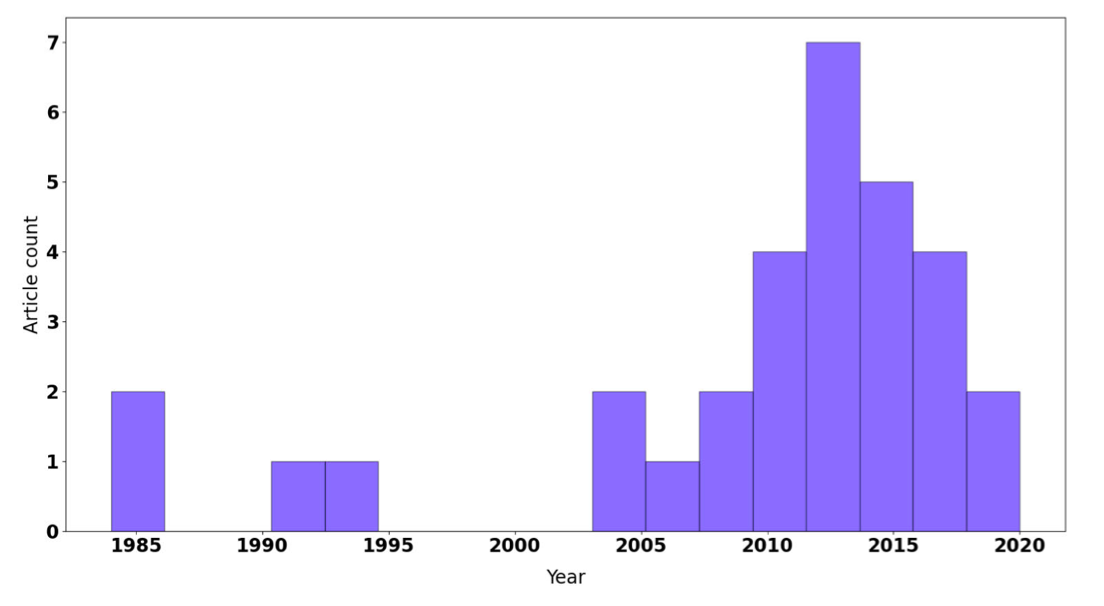
\includegraphics[width=0.9\textwidth]{Figures/publications.png}
	\label{fig:Distribution}
\end{figure}

\cite{GERBEC2005} tried to assign typical load profiles to a particular group of consumers based on their activity. 
To achieve that, they used probabilistic neural networks as a way of classification. Their methodology was tested in real use scenario. 

\cite{Gao2018} makes use of the bottom-up method to build a forecasting framework for household
load profiling, which takes into account the consumption patterns of residents. 
A model falls into the demand-side management subgroup.
They have developed a "single-day extraction model", designed to select the same days by comparing environmental and household factors, which influence energy consumption.
By using this approach, they have improved the accuracy of predicting behavioral patterns of dwellers. 
This method falls into the probabilistic method subgroup. Results show that their method successfully modeled daily usage.

\cite{Chuan2014} uses load profiling to optimize energy consumption distribution during the day.
This reduces peak usage and alleviates load off the grid. The author used the bottom-up method, that is, using sub-meter data.
Using this data, they made daily usage analyses on a one-hour basis. Using this information they optimized the daily activation of appliances
so that peak usage was not as high. Results show that peak shedding was successful. 

\cite{Csoknyai2019} analyzes energy consumption patterns and intervention strategies in residential buildings.
Authors achieve this using a "serious game approach" with a combination of direct user feedback using smart meters. 
The application also provides advice, comparisons, savings, reduction goals, and monitoring.
The approach takes into account almost all dimensions of residential energy usage. Their results show that their serious game was not
able to induce energy-saving behavior.

\cite{Jeong2021} used extreme points in the appliance usage curve to cluster usage profiles.
Usually, the first usage peak is in the morning, and the second one is in the evening. 
Additionally, they used demographic characteristics that are: region, area, age, salary, etc. to improve the results.
Using collected data, they clustered profiles. They had discovered 6 different usage profiles, 
where every cluster had a physical meaning such as energy-saving, morning heavy, evening heavy, etc.

Another clustering methodology was proposed by \cite{Park2019}, using load image profiles and image processing.
They represented time series data as an image. The image is a grid of squares where the y-axis contains monthly data with a resolution of one day,
x-axis contains daily data with a resolution of one hour. Grid is color filled with an algorithm that authors developed,
where red means more activity and blue less. Using digital image filters they transformed the type-1 image to type-2 and from there
used a threshold to obtain type-3. Using that information they clustered data based on images similarly. They used three different 
clustering methods: k-means, FCM, and EM algorithm. Using the Davies-Bouldin index, they were able to prove that image-based clustering performs better than non-image.

\cite{Joana2012} clustered different load profiles using electricity consumption data and surveys using data from residential homes.
They used PCA and k-means resulting in 5 clusters. Similar to other load profiling papers. 

Whereas most of the above-mentioned papers focused on aggregated consumption of building to build a load profile,
authors \cite{Issi2018} focused on appliance-level load profiling.
Their main contribution was to create a realistic per appliance load profile.
They developed a wireless measurement system with smart plugs that enabled them to obtain 
power signatures for each appliance. They evaluated the data and based on observations they determined working cycles for each appliance.
Furthermore, they concluded that 15 \% of consumed power can be shifted, where they took tariffs into account. 

\section{Anomaly detection in building energy consumption data}

A review on Anomaly detection in building energy consumption data was written by \cite{HIMEUR2021116601}.
Here, the authors took a deep dive into detecting anomalies in energy consumption in buildings. 
The author first makes an overview of existing anomaly detection schemes and applications.
Second, they perform a critical analysis and an in-depth discussion of the state-of-the-art.
Next, they describe current trends such as NILM anomaly detection. Finally, they assemble a set of future research directions. 
Both reviews pointed out that NILM anomaly detection or NILM load profiling is a possible future research direction.

\cite{NILMAD2019} authors propose an algorithm
that functions on top of existing state-of-the-art NILM algorithms Hidden Markov model,
combinatorial optimization, Latent Bayesian Modeling, and Graph-based Signal Processing.
They focus on three appliances, a fridge, freezer, and heater. Their metric was the number of operation cycles and energy used within those cycles. 
They implemented sigma variables to represent standard deviation and used rule-based anomaly detection.
So if energy or counts are significantly larger than the mean then the day is considered anomalous.
Their rule had only one manual setting and that was a number of standard deviations before the sample was considered anomalous.
Their results show that sub-meter anomaly detection works decently whereas NILM-based anomaly does not work at all. 

\cite{NILMAD22019} published another paper in the same year, where they took a similar approach, except that they used 
only compressor-based appliances such as fridges and air conditioners. They also added a rule to their existing rule-based anomaly 
detection algorithm, but the results still showed that NILM algorithms are not there yet. 

\cite{Castangia2021} used disaggregated sub-meter data to detect anomalies in use consumption.
They used a private dataset of 20 homes from northern Italy with no synthetic anomalies. 
Dataset included data from 2018 to 2020 meaning it included covid-induced anomalies. 
The authors first pre-processed the data by aggregating input load in hourly energy consumption, 
the second derived additional features, which are the time of use and duration of the activation.
They use that data to detect single-point deviations for which they implemented the isolation Forest algorithm and
anomalous trends for which to detect, they implemented Change Point Detection. 

\section{Example use-cases}
\label{sec:use-cases}

The load profiling method has a lot of different use cases across different fields.
In our case, we will split use cases into three classes.

The first class is grid management.
For example, it can be used to save energy by studying users' usage patterns and returning feedback.
Electrical energy providers could use that same data to optimize the management of their grid, with minimal impact on users' daily lives.

The second class is anomaly detection.
The load profiles could be used to help the elderly in case of an accident and help prevent one. 
They could be used to detect all kinds of early malfunctions in the operation of appliances and help save energy.

The last class is miscellaneous or other where occupancy detection, research, and development are all areas where profiling could be used. 

\subsection{Grid management}

\subsubsection{Zero energy buildings and energy saving}

As mentioned before many applications for load profiling could be used to reduce energy use and increase energy efficiency. 
With the emerging EV-market and ever-increasing installation of heat pumps, more and more energy is being used in form of electricity. 
This means, that most of the current power grids would have to be upgraded to keep up with demand.

On the other side, more and more photovoltaic systems are being installed,
which is slowly shifting energy production towards end-users.
Slowly energy grid is starting to shift towards so-called distributed energy resources or "DER" \cite{MORENOJARAMILLO2021445}.
DERs include all kinds of micro-energy sources such as PV, wind power, water power, and all kinds of energy accumulators that can store 
and release energy when needed such as heat pumps with hot water storage, home batteries, and EVs that can be used as a battery.

With smart management, these appliances could be used in a way that would reduce the net flow of energy and alleviate the load off the power grid.
A way to achieve this is via load profiling and load modeling. 
To manage the appliances, a control system would have to be put in place \cite{DirectLoadControll2021}.
It would be enough to control a few appliances that consume most of the energy. 

Since consumers take part in producing the energy, they are often called "prosumers" \cite{Prosumer2016}.
They will be an essential part of the European Union's plan to reach zero-energy buildings
and near-zero-energy buildings \cite{eu2021}. The directive was accepted in 2010 and was recast in 2021.
The plan is set to be realized in the next decade.

An actual use case would be an EV owner with an installed PV system and heat pump, who works from home on occasions.
In this case, two profiles would be developed. Normal workday and work from home day.
Additional information would be obtained from the users calendar. 
On a normal workday, the system would use PV energy to heat the water and store it, based on the user profile.
On work-from-home days, the system would start charging the car with the morning sun, using only the PV energy. 
In the evening hours, when consumption rises and production falls, EV could inject the power back into the house. 
Again using appliance load profiles to mitigate net energy flow as close to zero as possible (zero-energy building).
With the ever-increasing power capacity and increasing range of EVs, more and more battery capacity could be used for mitigation. 
In the case of grid batteries, similar steps could be taken.
This process is called vehicle-to-grid, and it is an important step towards zero-energy buildings \cite{EV2018} and \cite{EV2020}.

One other way to use user load profiles is to optimally distribute the load by studying users usage patterns as \cite{Chuan2014} and \cite{shift2015} proposed in their papers. 
This could be further extended to neighborhoods connected into peer 2 peer energy distribution networks.
As mentioned earlier, the way to save energy consumption is to distribute it as locally as possible. 
Knowing usage patterns of all peers, the system could optimally distribute the energy using DERs across all homes without dwellers even noticing.

Another use case could be using a heat pump and heat storage,
where besides users usage patterns system would also obtain weather forecasts from the internet.
Heat pumps that extract heat from the air are more efficient when temperature differences are smaller. 
The heat pump could store energy when warm and release the energy when cold.
Based on the user usage profile, energy could be optimally distributed.

Many papers have been published, where authors explored ways to reduce the energy consumption of users by studying user consumption patterns,
such as \cite{energy_saving3}, \cite{energy_saving1}, \cite{energy_saving4} and \cite{energy_saving3}.
Energy saving is done through instant feedback, reduction goals, rewards, and by comparing their user profile to the average user as the authors did in \cite{Csoknyai2019}.
Source \cite{eu2006} states that as much as 20 \% of energy could be saved by managing the consumption.

\subsubsection{Demand response}

An increasing percentage of renewable resources is troubling energy distributors, due to the nature of renewable resources.
In the prior chapter, it was mentioned how energy-saving measures would benefit users and their peers.
One other use case would be cooperation between end-user and energy distribution companies.
Joint actions between them would benefit both as authors show in \cite{cooperation2008} and \cite{cooperation2010}

The electricity provider could control the main appliances so that load on the power grid is uniform,
with as few peaks and valleys as possible. For this to function, users would have to allow the installation of energy meters and controllers 
on appliances that use the most electricity \cite{gridDirectControll2015}. One way to achieve this is to control the voltage of loads \cite{controll2014} the other
way is to shift the loads in time \cite{shift2015}.
This process is called direct load control \cite{DirectLoadControll2021}, and it is part of demand response program \cite{DemandResponse2018}.

"DR program is a voluntary PJM program that compensates end-use (retail) customers for reducing their electricity use (load)
when requested by PJM during periods of high power prices, or when the reliability of the grid is threatened." \cite{DemandResponse2018}

The benefit to the user would be lower the cost of charging EVs and heating the building.
This is already done through so-called small and high tariffs.
More detailed user load profiles would enable the electricity provider to introduce real-time tariffs to the user.

The user would have three options. The first one would be that users can use the appliances as freely as they desire, this would result in a normal tariff.
The second option would be to use the appliances as regularly as possible, this would lead to lower tariffs.
The third option would be to leave the management of main appliances to the electricity provider.
The provider would combine the user appliance load profile and the real-time market price of energy to optimize the cost \cite{optimiseCostShift2015}.
This would lead to free or even negative prices of electricity since distribution companies have to keep the frequency of the grid as stable as possible.

For them to stabilize the frequency, they sometimes have to resort to load shedding.
Load shedding is a process where a load is disconnected from the grid to keep the grid in sync \cite{loadShedding2006}.
Commonly whole neighborhoods are being disconnected, affecting their daily lives.
Using user load profiles, distribution companies could disconnect the load in a way that would minimally affect the end-user. 
When they would need to load the grid due to low demand, they could charge EVs free of charge or even pay to do so. 
This benefits the company as well since they do not need to lower energy production, which can be expensive. 

\subsection{Anomaly detection}

One use case of anomaly detection was already mentioned in the Elderly care chapter.
One more thing that could be detected, using load profiling, would be the altered operation of appliances.
In the case of a fridge, the system would detect that duty cycles are too long.
The increased duty cycle can be caused by cooling liquid leakage, fridge being open or compressor motor malfunction.
Heat pumps work on the same basis as fridges, meaning the same anomalies could be detected. 
The malfunction could also be detected in heating element appliances such as toasters or boilers. 
Since mentioned appliances are one of the largest consumers in a household,
early enough detection could lead to large energy-saving benefits \cite{NILMAD2019}.

\subsubsection{Elderly care}

Demographic changes i.e. aging population is an increasing socioeconomic issue.
The elderly are facing many issues when staying at home alone for extended periods.
Accidents such as falls or the inability to do choirs due to health-related issues or even dementia-induced issues 
such as leaving appliances on for long periods could all be detected, using sub-meter data such as authors \cite{elder1} and \cite{elder2}
explore in their papers.

To detect falls or other issues a normal daily appliance use profile would be developed.
It would involve routine behavior of users such as turning on the coffee machine in the morning, the stove and oven at the noon or using the toaster in the evening.
All these routines could be measured and tracked. Using this data, a profile would be developed.
The probability of an anomaly and a threshold would enable the system to detect an issue.

An example would be: the coffee machine not turning on in the morning or the stove and kitchen vent not being used at the noon.
Another issue could be detected if the appliance would be used more frequently or for extended periods of time. 
This could indicate that the user forgot to turn off the stove, oven, or even a light. The same system could detect 
that a fridge or a freezer was left open since the duty cycles would be longer and more frequent. 
As soon as the issue would be detected it would notify the caregiver to check on the patient.

\subsection{Other}

Load profiling could also be used as feedback for the engineers and designers,
of how a certain device is being used and if it is being used as designed. 
This would enable the manufacturers to improve their products according to 
user's needs, without unnecessary features.

\cite{energyStealing2018} uses anomaly detection algorithms and load profiling to detect energy lost due to non-technical losses.
This occurs after the smart-meter is exposed to cyber or mechanical attacks and its measurements are off. 

One other use case could be occupancy detection of buildings such as the authors explore in \cite{occupancy2013}. Information about 
occupancy could be used as part of elderly care monitoring or in the case of building
automation, to run certain tasks when a user enters or leaves the room or a building.

